\section{R-CNN, Fast R-CNN, Faster R-CNN}
Previous architectures I was talking about served for solving classification (AlexNet, DenseNet, ResNet) or segmentation tasks (UNet). Another computer vision problem is object detection - finding instances of objects of classes in an image. That means localizing several objects of several classes withing one image.

R-CNN \cite{rcnn2014} (R stands for regions) proposed a method which combines region proposals and CNNs. Region proposals are a set of ``sub-images'' for classification. These regions are chosen by selective search. R-CNN architecture consists of 3 modules \ref{fig:rcnn}: First module takes the input image and generates around 2000 region proposals. These are then fed to a CNN which computes feature maps for them. And the last module is a linear SVM, which classifies the regions.

\begin{figure}[ht!]
    \centering
    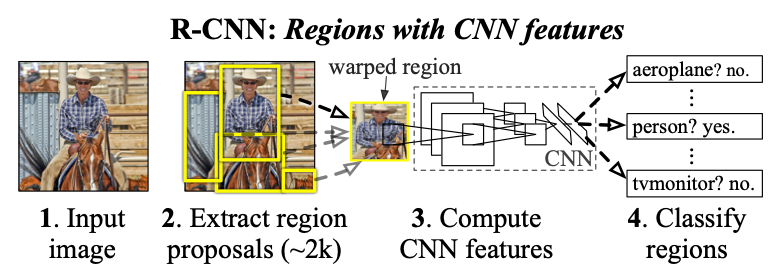
\includegraphics[width=200pt]{images/r-cnn.png}
    \caption[R-CNN modules]{R-CNN modules \cite{rcnn2014}}
    \label{fig:rcnn}
\end{figure}

The problem with R-CNN is that it is slow. This problem stems from the use of selective search to produce proposals, which are processed by CNN one by one . Therefore, its author came up with another method to speed up the process, Fast R-CNN \cite{fast-rcnn2015}. Input for this network is the whole image and a set of proposals. Generated convolutional maps are passed to the ROI (region of interest) pooling layer. This layer resizes them to a fixed size, so they can be fed into a fully connected layer. Squeezing an image and its proposals together reduces the number of convolutional passes and makes the whole process faster. 

Even faster version called Faster R-CNN was developed \cite{faster-rcnn2017}. Instead of using selective search to exhaustively produce region proposals, a Region Proposal Network is introduced. It is a fully convolutional network, which takes an image of any size as its input and outputs predictded object bounds. Those are then passed to the ROI pooling layer and then classified. 